\documentclass{article}

%
% 引入模板的style文件
%
\usepackage{homework}

\setCJKmainfont{SimSun}[AutoFakeBold] %宋体加粗
\setCJKsansfont{SimHei}[AutoFakeBold] %黑体加粗


\usepackage{minted} %配合minted宏包进行好看的高亮
\usepackage{currfile} %配合minted宏包进行好看的高亮
\usepackage{caption} %配合minted宏包进行好看的高亮
\usepackage{tcolorbox} %配合minted宏包进行好看的高亮
\usepackage{xcolor} %配合minted宏包进行好看的高亮
\tcbuselibrary{skins} %配合minted宏包进行好看的高亮
\tcbuselibrary{minted} %配合minted宏包进行好看的高亮
\usemintedstyle{paraiso-dark} %配合minted宏包进行好看的高亮



%
% 封面
%

\title{
	
\includegraphics[width=0.6\textwidth]{images/title/ucas_logo 1.pdf}\\
    \vspace{1in}
    \textmd{\textbf{\hmwkClass}}\\
	\textmd{\Large{\textbf{\hmwkClassID}}}\\
    \textmd{\textbf{\hmwkTitle}}\\
    \normalsize\vspace{0.1in}\large{\hmwkCompleteTime }\\
    \vspace{0.1in}\large{\textit{\hmwkClassInstructor\ }}\\
    \vspace{1in}
	
\includegraphics[width=0.25\textwidth]{images/title/Cyber.jpg}\\
	\vspace{1in}
}


\author{
	\hmwkAuthorName \\ 
	\hmwkAuthorStuID \\
	\hmwkAuthorInst \\
	\hmwkAuthorzhuanye \\
	\hmwkAuthorfangxiang
	}
\date{}

\renewcommand{\part}[1]{\textbf{\large Part \Alph{partCounter}}\stepcounter{partCounter}\\}


%
% 正文部分
%
\begin{document}


\maketitle


%\include{chapters/ch01}
%\include{chapters/ch02}
%\include{chapters/ch03}
%\include{chapters/ch04}
%\include{chapters/ch05}




\begin{homeworkProblem}
	给定如下训练数据集$$\boldsymbol{X}=\left( \begin{matrix}
		3&		4&		1\\
		3&		3&		1\\
	\end{matrix} \right) ,\boldsymbol{y}=\left( \begin{matrix}
		1&		1&		-1\\
	\end{matrix} \right) ^{\text{T}}$$
	通过求解SVM的\textbf{原始问题}来求解最大间隔的分离超平面.
	\\

	\solution 通过求解如下最优化问题来得到最优分类器的参数$\left( \boldsymbol{w}^{\ast},b^{\ast} \right)$:
	$$
	\begin{cases}
		\displaystyle \underset{\boldsymbol{w},b}{\text{min}}\,\,\frac{1}{2}\left\| \boldsymbol{w} \right\| _{2}^{2}\\
		\text{s}.\text{t}.\,\, y^{\left( i \right)}\left( \boldsymbol{w}^{\text{T}}\boldsymbol{x}^{\left( i \right)}+b \right) \ge 1,i=1,\cdots ,N\\
	\end{cases}\Rightarrow 
	\begin{cases}
		\displaystyle \underset{\left( w_1,w_2 \right) ,b}{\text{min}}\,\,\frac{1}{2}\left( w_{1}^{2}+w_{2}^{2} \right)\\
		3w_1+3w_2+b\ge 1\\
		4w_1+3w_2+b\ge 1\\
		-\left( w_1+w_2+b \right) \ge 1\\
	\end{cases}
	$$
	要求求解这个严格的凸二次规划问题, 我们可以直接利用Matlab中的二次规划问题求解包直接求解. 而二次规划的标准形式为
	$$
	\begin{cases}
		\displaystyle \underset{\boldsymbol{x}}{\text{min}}\,\,\frac{1}{2}\boldsymbol{x}^{\text{T}}\boldsymbol{Hx}+\boldsymbol{f}^{\text{T}}\boldsymbol{x}\\
		\boldsymbol{A}\cdot \boldsymbol{x}\le \boldsymbol{b}\\
	\end{cases}
	$$
	对照过来, 可以知道
	$$
	\boldsymbol{H}=\left( \begin{matrix}
		1&		0&		0\\
		0&		1&		0\\
		0&		0&		0\\
	\end{matrix} \right) , \boldsymbol{f}=\left( \begin{array}{c}
		0\\
		0\\
		0\\
	\end{array} \right) , \boldsymbol{A}=\left( \begin{matrix}
		-3&		-3&		-1\\
		-4&		-3&		-1\\
		1&		1&		1\\
	\end{matrix} \right) , \boldsymbol{b}=\left( \begin{array}{c}
		-1\\
		-1\\
		-1\\
	\end{array} \right)
	$$
	于是我们可以在Matlab中写出如下代码:
\begin{tcblisting}{listing engine=minted,boxrule=0.1mm,
colback=blue!5!white,colframe=blue!75!black,
listing only,left=5mm,enhanced,sharp corners=all,
overlay={\begin{tcbclipinterior}\fill[red!20!blue!20!white] (frame.south west)
rectangle ([xshift=5mm]frame.north west);\end{tcbclipinterior}},
minted language=matlab,
minted style=tango,
minted options={fontsize=\normalsize,breaklines,autogobble,linenos,numbersep=3mm}}
H = [1, 0, 0; 0, 1, 0; 0, 0, 0];
f = [0; 0; 0];
A = [-3, -3, -1; -4, -3, -1; 1, 1, 1];
b = [-1; -1; -1];
[x, fval, exitflag, output, lambda] = quadprog(H, f, A, b)
\end{tcblisting}
	执行后便可得到结果(exitflag=1, 即问题存在最优解):
	$$
	\boldsymbol{x}^{\ast}=\left( \begin{array}{c}
		w_{1}^{\ast}\\
		w_{2}^{\ast}\\
		b^{\ast}\\
	\end{array} \right) =\left( \begin{array}{c}
		0.5\\
		0.5\\
		-2\\
	\end{array} \right) , \displaystyle \underset{\left( w_1,w_2,b \right)}{\text{min}}\,\,\frac{1}{2}\left( w_{1}^{2}+w_{2}^{2} \right) =0.25
	$$
	于是最大间隔的分离超平面方程和判别函数分别为$$\frac{1}{2}x_1+\frac{1}{2}x_2-2=0, f_{\boldsymbol{w},b}\left( \boldsymbol{x} \right) =\text{sgn} \left( \frac{1}{2}x_1+\frac{1}{2}x_2-2 \right) 
	$$
	本题的训练样本较少, 所以方法2是说: 可以直接观察出支持向量(而不用求解上述二次规划问题), 从而立即得到具有最大间隔的分离超平面\footnote{这是因为最终模型仅与\textbf{支持向量}有关.}. 具体如下图\ref{fig:最大间隔分离超平面示意图}所示:
	\newpage
	\begin{figure}[H]  % 这里记得用[H]
		\centering
		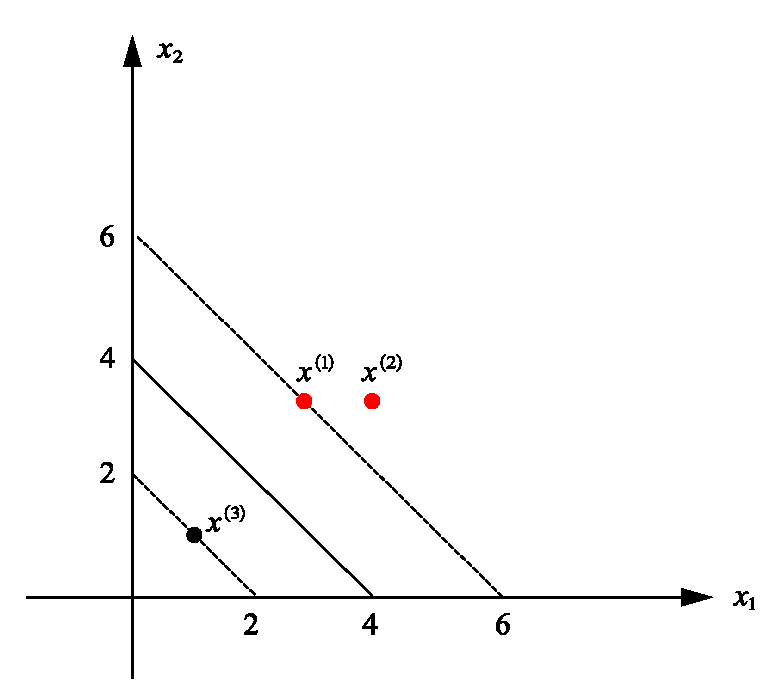
\includegraphics[width=0.6\textwidth]{images/title/最大间隔分离超平面示意图.pdf}
		\caption{最大间隔分离超平面示意图}
		\label{fig:最大间隔分离超平面示意图}
	\end{figure}
	明显可以看出支持向量为$x^{(3)},x^{(1)}$, 所以\textbf{这两个点的垂直平分线就是所要求的最大间隔分离超平面}! 即其方程为$0.5x_1+0.5x_2-2=0$.
	而对于上述二次优化问题, 我们也可以利用拉格朗日数乘法求解如下: 构造辅助函数(只代入支持向量, 因为最终模型只与支持向量有关)
	$$
	L\left( \boldsymbol{w},b,\boldsymbol{\alpha } \right) =\frac{1}{2}\left( w_{1}^{2}+w_{2}^{2} \right) +\alpha _1\left( 1-3w_1-3w_2-b \right) +\alpha _2\left( 1+w_1+w_2+b \right) 
	$$
	对$w_1,w_2,b$分别求偏导:
	$$
	\begin{cases}
		w_1-3\alpha _1+\alpha _2=0\\
		w_2-3\alpha _1+\alpha _2=0\\
		-\alpha _1+\alpha _2=0\\
	\end{cases}\Rightarrow w_1=w_2=2\alpha _1
	$$
	代入辅助函数可得:$$L\left( \alpha _1 \right) =-4\alpha _{1}^{2}+2\alpha _1, L'\left( \alpha _1 \right) =-8\alpha _1+2
	$$
	令$L'(\alpha_1)=0$得$\displaystyle \alpha_1=\frac{1}{4}$, 因此$\displaystyle w_1=w_2=\frac{1}{2}$, 从而$b\leq -2$, 于是最大间隔的分离超平面方程为$$\frac{1}{2}x_1+\frac{1}{2}x_2-2=0$$
\end{homeworkProblem}


\pagebreak


\begin{homeworkProblem}
	给定如下训练数据集$$\boldsymbol{X}=\left( \begin{matrix}
		3&		4&		1\\
		3&		3&		1\\
	\end{matrix} \right) ,\boldsymbol{y}=\left( \begin{matrix}
		1&		1&		-1\\
	\end{matrix} \right) ^{\text{T}}$$
	通过求解SVM的\textbf{对偶问题}来求解最大间隔的分离超平面.
	\\

	\solution \,\,SVM的对偶问题为
	$$
	\begin{cases}
		\displaystyle \underset{\boldsymbol{\alpha }}{\text{max}}\left\{ \sum_{i=1}^N{\alpha _i}-\frac{1}{2}\sum_{i,j=1}^N{\alpha _i\alpha _jy^{\left( i \right)}y^{\left( j \right)}\left< \boldsymbol{x}^{\left( i \right)},\boldsymbol{x}^{\left( j \right)} \right>} \right\}\\
		\text{s.t.}\,\, \alpha _i\ge 0,i=1,\cdots ,N\\
		\displaystyle \sum_{i=1}^N{\alpha _iy^{\left( i \right)}}=0\\
	\end{cases}
	$$
	代入上述训练样本具体化对偶问题可得
	$$
	\begin{cases}
		\displaystyle \underset{\boldsymbol{\alpha }}{\text{max}}\left\{ \sum_{i=1}^3{\alpha _i}-\frac{1}{2}\left( 18\alpha _{1}^{2}+25\alpha _{2}^{2}+2\alpha _{3}^{2}+21\alpha _1\alpha _2-6\alpha _1\alpha _3-7\alpha _2\alpha _3 \right) \right\}\\
		\alpha _i\ge 0,i=1,2,3\\
		\alpha _1+\alpha _2-\alpha _3=0\\
	\end{cases}
	$$
	而求解这个二次规划问题, 我们可以利用Matlab中的求解包来求解. 而二次规划的标准形式为
	$$
	\begin{cases}
		\displaystyle \underset{\boldsymbol{x}}{\text{min}}\,\,\frac{1}{2}\boldsymbol{x}^{\text{T}}\boldsymbol{Hx}+\boldsymbol{f}^{\text{T}}\boldsymbol{x}\\
		\boldsymbol{A}\cdot \boldsymbol{x}\le \boldsymbol{b}\\
		\boldsymbol{A}_{eq}\cdot \boldsymbol{x}=\boldsymbol{b}_{eq}\\
	\end{cases}
	$$
	对照过来可以知道:
	\begin{align}
		\boldsymbol{H}&=\left( \begin{matrix}
			18&		10.5&		-3\\
			10.5&		25&		-3.5\\
			-3&		-3.5&		2\\
		\end{matrix} \right) ,\boldsymbol{f}=\left( \begin{array}{c}
			-1\\
			-1\\
			-1\\
		\end{array} \right) \notag
		\\
		\boldsymbol{A}&=\left( \begin{matrix}
			-1&		0&		0\\
			0&		-1&		0\\
			0&		0&		-1\\
		\end{matrix} \right) ,\boldsymbol{b}=\left( \begin{array}{c}
			0\\
			0\\
			0\\
		\end{array} \right), \boldsymbol{A}_{eq}=\left( \begin{matrix}
			1&		1&		-1\\
		\end{matrix} \right) ,\boldsymbol{b}_{eq}=\left( 0 \right) \notag
	\end{align}
	于是我们可以在Matlab中写出如下代码:
\begin{tcblisting}{listing engine=minted,boxrule=0.1mm,
colback=blue!5!white,colframe=blue!75!black,
listing only,left=5mm,enhanced,sharp corners=all,
overlay={\begin{tcbclipinterior}\fill[red!20!blue!20!white] (frame.south west)
rectangle ([xshift=5mm]frame.north west);\end{tcbclipinterior}},
minted language=matlab,
minted style=tango,
minted options={fontsize=\normalsize,breaklines,autogobble,linenos,numbersep=3mm}}
H = [18, 10.5, -3; 10.5, 25, -3.5; -3, -3.5, 2];
f = [-1; -1; -1];
A = [-1, 0, 0; 0, -1, 0; 0, 0, -1];
b = [0; 0; 0];
A_eq = [1, 1, -1];
b_eq = [0];
[x, fval, exitflag, output, lambda] = quadprog(H, f, A, b, A_eq, b_eq)
\end{tcblisting}
	根据代码输出就可以得到对偶问题的最优解$\boldsymbol{\alpha}^{\ast}$和相应的最优值分别为
	$$
	\boldsymbol{\alpha }^{\ast}=\left( \begin{array}{c}
		0.25\\
		0\\
		0.25\\
	\end{array} \right) , \underset{\boldsymbol{\alpha }}{\text{max}}\left\{ \sum_{i=1}^3{\alpha _i}-\frac{1}{2}\left( 18\alpha _{1}^{2}+25\alpha _{2}^{2}+2\alpha _{3}^{2}+21\alpha _1\alpha _2-6\alpha _1\alpha _3-7\alpha _2\alpha _3 \right) \right\} =0.0625
	$$
	于是原问题的最优解$\left( \boldsymbol{w}^{\ast}, b^{\ast} \right)$为
	\begin{align}
		\displaystyle \boldsymbol{w}^{\ast}&=\sum_{i=1}^N{\alpha _{i}^{\ast}y^{\left( i \right)}\boldsymbol{x}^{\left( i \right)}}=0.25\cdot \left( \begin{array}{c}
			3\\
			3\\
		\end{array} \right) +0\cdot \left( \begin{array}{c}
			4\\
			3\\
		\end{array} \right) -0.25\cdot \left( \begin{array}{c}
			1\\
			1\\
		\end{array} \right) =\left( \begin{array}{c}
			0.5\\
			0.5\\
		\end{array} \right) \notag
		\\
		\displaystyle b^{\ast}&=y^{\left( j \right)}-\sum_{i=1}^N{\alpha _{i}^{\ast}y^{\left( i \right)}\left< \boldsymbol{x}^{\left( i \right)},\boldsymbol{x}^{\left( j \right)} \right>},\alpha _{j}^{\ast}>0\Rightarrow b^{\ast}=y^{\left( 1 \right)}-\sum_{i=1}^3{\alpha _{i}^{\ast}y^{\left( i \right)}\left< \boldsymbol{x}^{\left( i \right)},\boldsymbol{x}^{\left( 1 \right)} \right>}=-2 \notag
	\end{align}
	于是分离超平面方程和判别函数的表达式分别为$${\boldsymbol{w}^{\ast}}^{\text{T}}\boldsymbol{x}+b^{\ast}=0.5\left( x_1+x_3 \right) -2=0, f_{\boldsymbol{w},b}\left( \boldsymbol{x} \right) =\text{sgn} \left( {\boldsymbol{w}^{\ast}}^{\text{T}}\boldsymbol{x}+b^{\ast} \right) 
	$$
	对于上面的对偶问题, 我们也可以解析求解: 根据约束条件可知$\alpha _3=\alpha _1+\alpha _2$, 代入目标函数可得$$\theta _D\left( \alpha _1,\alpha _2 \right) =-4\alpha _{1}^{2}-10\alpha _1\alpha _2-3\alpha _{2}^{2}+2\alpha _1+2\alpha _2
	$$
	于是$$\frac{\partial \theta _D\left( \alpha _1,\alpha _2 \right)}{\partial \alpha _1}=-8\alpha _1-10\alpha _2+2=0\Rightarrow \alpha _1=\frac{1}{4}-\frac{5\alpha _2}{4}
	$$
	代入$\theta_D(\alpha_1,\alpha_2)$可得
	$$
	\theta _D\left( \alpha _2 \right) =-\frac{1}{4}\alpha _{2}^{2}-\frac{1}{2}\alpha _2+\frac{1}{4}\xrightarrow{\alpha _2\ge 0}\underset{\alpha _2\ge 0}{\text{max}}\theta _D=\theta _D\left( 0 \right) =\frac{1}{4}\Rightarrow a_2=0,\alpha _1=\alpha _3=\frac{1}{4}
	$$
	对于原问题最优解的推导与上面的过程一致, 就不赘述了. 我们也可以利用下述的算法\ref{alg:SMO}(即SMO算法)来求出SVM的对偶问题的解为$\boldsymbol{\alpha}^{\ast}=(0.25,0,0.25)^{\text{T}}$:
	\begin{algorithm}[H]
		\begin{algorithmic}[1]
		\Require{训练数据集$S=\left\{ \left( \boldsymbol{x}^{\left( i \right)},y^{\left( i \right)} \right) ,i=1,\cdots ,N \right\}$, 误差$\epsilon$}
		\Ensure{$\hat{\alpha}=\left( \hat{\alpha}_1,\cdots ,\hat{\alpha}_N \right)$}
		\State 初始化: $\alpha^{(0)}\gets 0,k\gets 0, C\gets +\infty$, 并计算偏移量$b^{(0)}$;
		\State 初始化误差项: $E_i\gets g\left( \boldsymbol{x}^{\left( i \right)} \right) -y^{\left( i \right)}$;
		\While{不满足KKT条件且$\exists i\in \left\{1,2,\cdots,N\right\},\,\text{s.t.}\,E_i\geq \epsilon$}
			\State $k\gets k+1$并选择待优化的变量: $\alpha _{1}^{\left( k \right)},\alpha _{2}^{\left( k \right)}$, 然后求解优化问题的解$\alpha _{1}^{\left( k+1 \right)},\alpha _{2}^{\left( k+1 \right)}$:
			\begin{align}
				&\alpha _{2}^{\text{new},\text{unclipped}}\gets \alpha _{2}^{\left( k \right)}+\frac{y^2\left( E_1-E_2 \right)}{\eta},,\,\,\alpha _{2}^{\left( k+1 \right)}\gets \begin{cases}
					H,&		\text{若}\alpha _{2}^{\text{new},\text{unclipped}}>H\\
					\alpha _{2}^{\text{new},\text{unclipped}},&		\text{若}L\le \alpha _{2}^{\text{new},\text{unclipped}}\le H\\
					L,&		\text{若}\alpha _{2}^{\text{new},\text{unclipped}}<L\\
				\end{cases} \notag
				\\
				&\eta \gets K_{11}+K_{22}-2K_{12}, \,\,\, \alpha _{1}^{\left( k+1 \right)}\gets \alpha _{1}^{\left( k \right)}+y^{\left( 1 \right)}y^{\left( 2 \right)}\left( \alpha _{2}^{\left( k \right)}-\alpha _{2}^{\left( k+1 \right)} \right) \notag	
			\end{align}
			\State 更新$\alpha \gets \alpha^{(k+1)}$, 更新$E_i\gets g\left( \boldsymbol{x}^{\left( i \right)} \right) -y^{\left( i \right)}	$, 计算$b^{(k+1)}$;
		\EndWhile
		\State \textbf{end \{SMO\}}
		\end{algorithmic}
		\caption{\textbf{SMO}算法}
		\label{alg:SMO}
	\end{algorithm}
\end{homeworkProblem}

\pagebreak


\begin{homeworkProblem}
	推导软间隔SVM的对偶形式.
	\\

	\solution 软间隔分类器SVM的原问题如下:
	$$
	\begin{cases}
		\displaystyle \underset{\boldsymbol{w},b}{\text{min}}\,\,\frac{1}{2}\left\| \boldsymbol{w} \right\| _{2}^{2}+C\sum_{i=1}^N{\xi _i}\\
		y^{\left( i \right)}\left( \boldsymbol{w}^{\text{T}}\boldsymbol{x}^{\left( i \right)}+b \right) \ge 1-\xi _i,i=1,\cdots ,N\\
		\xi _i\ge 0,i=1,\cdots ,N\\
	\end{cases}
	$$
	于是我们可以构造如下的广义拉格朗日函数:
	$$
	L\left( \boldsymbol{w},b,\boldsymbol{\xi },\boldsymbol{\alpha },\boldsymbol{\eta } \right) =\frac{1}{2}\left\| \boldsymbol{w} \right\| _{2}^{2}+C\sum_{i=1}^N{\xi _i}-\sum_{i=1}^N{\alpha _i\left[ y^{\left( i \right)}\left( \boldsymbol{w}^{\text{T}}\boldsymbol{x}^{\left( i \right)}+b \right) -1+\xi _i \right]}-\sum_{i=1}^N{\eta _i\xi _i}
	$$
	先固定拉格朗日乘子$\boldsymbol{\alpha},\boldsymbol{\eta}$, 关于$\boldsymbol{w},b,\xi_i$对$L\left( \boldsymbol{w},b,\boldsymbol{\xi },\boldsymbol{\alpha },\boldsymbol{\eta } \right)$做优化(最小化)得到$\theta_D(\boldsymbol{\alpha},\boldsymbol{\eta})$:
	$$
	\begin{cases}
		\displaystyle \nabla _{\boldsymbol{w}}L\left( \boldsymbol{w},b,\boldsymbol{\xi },\boldsymbol{\alpha },\boldsymbol{\eta } \right) =\boldsymbol{w}-\sum_{i=1}^N{\alpha _iy^{\left( i \right)}\boldsymbol{x}^{\left( i \right)}}=0\\
		\displaystyle \frac{\partial}{\partial b}L\left( \boldsymbol{w},b,\boldsymbol{\xi },\boldsymbol{\alpha },\boldsymbol{\eta } \right) =-\sum_{i=1}^N{\alpha _iy^{\left( i \right)}}=0\\
		\displaystyle \frac{\partial}{\partial \xi _i}L\left( \boldsymbol{w},b,\boldsymbol{\xi },\boldsymbol{\alpha },\boldsymbol{\eta } \right) =C-\alpha _i-\eta _i=0\\
	\end{cases}
	$$
	将上述3个条件代入广义拉格朗日函数可得到$\theta_D(\boldsymbol{\alpha},\boldsymbol{\eta})$:
	\begin{align}
		\theta _D\left( \boldsymbol{\alpha },\boldsymbol{\eta } \right) &=\frac{1}{2}\boldsymbol{w}^{\text{T}}\boldsymbol{w}+C\sum_{i=1}^N{\xi _i}-\sum_{i=1}^N{\alpha _i\left[ y^{\left( i \right)}\left( \boldsymbol{w}^{\text{T}}\boldsymbol{x}^{\left( i \right)}+b \right) -1+\xi _i \right]}-\sum_{i=1}^N{\eta _i\xi _i} \notag
		\\
		&=\frac{1}{2}\sum_{i=1}^N{\alpha _iy^{\left( i \right)}\left( \boldsymbol{x}^{\left( i \right)} \right) ^{\text{T}}}\sum_{j=1}^N{\alpha _jy^{\left( j \right)}\boldsymbol{x}^{\left( j \right)}}-\sum_{i=1}^N{\alpha _i\left[ y^{\left( i \right)}\left( \sum_{j=1}^N{\alpha _jy^{\left( j \right)}\left( \boldsymbol{x}^{\left( j \right)} \right) ^{\text{T}}\boldsymbol{x}^{\left( i \right)}}+b \right) -1+\xi _i \right]} \notag
		\\
		&+C\sum_{i=1}^N{\xi _i}-\sum_{i=1}^N{\eta _i\xi _i} \notag
		\\
		&=\frac{1}{2}\sum_{i,j=1}^N{\alpha _i\alpha _jy^{\left( i \right)}y^{\left( j \right)}\left< \boldsymbol{x}^{\left( i \right)},\boldsymbol{x}^{\left( j \right)} \right>}-\sum_{i,j=1}^N{\alpha _i\alpha _jy^{\left( i \right)}y^{\left( j \right)}\left< \boldsymbol{x}^{\left( i \right)},\boldsymbol{x}^{\left( j \right)} \right>} -b\cdot \sum_{i=1}^N{\alpha _iy^{\left( i \right)}} \notag
		\\
		&+\sum_{i=1}^N{\alpha _i}+\sum_{i=1}^N{\left( C-\alpha _i-\eta _i \right) \xi _i} \notag
		\\
		&=-\frac{1}{2}\sum_{i,j=1}^N{\alpha _i\alpha _jy^{\left( i \right)}y^{\left( j \right)}\left< \boldsymbol{x}^{\left( i \right)},\boldsymbol{x}^{\left( j \right)} \right>}+\sum_{i=1}^N{\alpha _i} \notag
	\end{align}
	即得到$$\theta _D\left( \boldsymbol{\alpha },\boldsymbol{\eta } \right) =\underset{\boldsymbol{w},b,\xi}{\text{min}}L\left( \boldsymbol{w},b,\boldsymbol{\xi },\boldsymbol{\alpha },\boldsymbol{\eta } \right) =\sum_{i=1}^N{\alpha _i}-\frac{1}{2}\sum_{i,j=1}^N{\alpha _i\alpha _jy^{\left( i \right)}y^{\left( j \right)}\left< \boldsymbol{x}^{\left( i \right)},\boldsymbol{x}^{\left( j \right)} \right>}=\theta _D\left( \boldsymbol{\alpha } \right) 
	$$
	于是最大化$\theta_D(\boldsymbol{\alpha})$, 即可得出下述的对偶问题:
	$$
	\begin{cases}
		\displaystyle \underset{\boldsymbol{\alpha }}{\text{max}}\left\{ \sum_{i=1}^N{\alpha _i}-\frac{1}{2}\sum_{i,j=1}^N{\alpha _i\alpha _jy^{\left( i \right)}y^{\left( j \right)}\left< \boldsymbol{x}^{\left( i \right)},\boldsymbol{x}^{\left( j \right)} \right>} \right\}\\
		\displaystyle \sum_{i=1}^N{\alpha _iy^{\left( i \right)}}=0\\
		0\le \alpha _i=\underset{\because \eta _i\ge 0\left( \text{乘子非负} \right)}{\underbrace{C-\eta _i\le C}},i=1,\cdots ,N\\
	\end{cases}
	$$
	假设$\boldsymbol{\alpha }^{\ast}=\left( \alpha _{1}^{\ast},\cdots ,\alpha _{N}^{*} \right)$是上述对偶问题的最优解, 那么原问题的解可以如下求解:
	显然$\boldsymbol{w}^{\ast}$可以直接写出:
	$$
	\boldsymbol{w}^{\ast}=\sum_{i=1}^N{\alpha _{i}^{\ast}y^{\left( i \right)}\boldsymbol{x}^{\left( i \right)}}
	$$
	而对于$b^{\ast}$, 需要找到一个相关的等式, 而根据库恩塔克条件(KKT)可得$$\alpha _i\left[ y^{\left( i \right)}\left( \boldsymbol{w}^{\text{T}}\boldsymbol{x}^{\left( i \right)}+b \right) -1+\xi _i \right] =0,\eta _i\xi _i=0
	$$
	因此若想要得到$b$的等式, 则根据互补松弛性可知, 只需要$\alpha_i>0(\neq 0)$, 但是$\xi_i$又是不能知道的, 所以需要想办法把它去掉(即需要使得$\xi_i=0$), 于是又根据互补松弛性可知, 再需要令$\eta_i>0(\neq 0)$即可使得$\xi_i=0$, 从而可得出$b$的等式$$y^{\left( i \right)}\left( \boldsymbol{w}^{\text{T}}\boldsymbol{x}^{\left( i \right)}+b \right) =1\Rightarrow b=y^{\left( i \right)}-\boldsymbol{w}^{\text{T}}\boldsymbol{x}^{\left( i \right)}
	$$
	因此若想求得$b^{\ast}$, 则需要挑选样本$\left(\boldsymbol{x}^{(j)},y^{(j)}\right)$, 使得样本满足$\alpha_j^{\ast}>0,\eta_j>0$ (即${\color{red} 0<\alpha_j^{\ast}<C}$), 于是可求得
	$$
	b^{\ast}=y^{\left( j \right)}-\boldsymbol{w}^{\text{T}}\boldsymbol{x}^{\left( j \right)}=y^{\left( j \right)}-\sum_{i=1}^N{\alpha _{i}^{\ast}y^{\left( i \right)}\left( \boldsymbol{x}^{\left( i \right)} \right) ^{\text{T}}\boldsymbol{x}^{\left( j \right)}}=y^{\left( j \right)}-\sum_{i=1}^N{\alpha _{i}^{\ast}y^{\left( i \right)}\left< \boldsymbol{x}^{\left( i \right)},\boldsymbol{x}^{\left( j \right)} \right>}
	$$
	于是可求得分类超平面方程和判别函数分别为$$\left( \boldsymbol{w}^{\ast} \right) ^{\text{T}}\boldsymbol{x}+b^{\ast}=0, f_{\boldsymbol{w},b}\left( \boldsymbol{x} \right) =\text{sgn} \left\{ \left( \boldsymbol{w}^{\ast} \right) ^{\text{T}}\boldsymbol{x}+b^{\ast} \right\} 
	$$
\end{homeworkProblem}


\pagebreak

\begin{homeworkProblem}
	高斯核的形式如下
	$$
	\mathcal{K}\left( \boldsymbol{x},\boldsymbol{z} \right) =\text{exp} \left( -\frac{\left\| \boldsymbol{x}-\boldsymbol{z} \right\| ^2}{2\sigma ^2} \right) 
	$$
	请证明高斯核可以表示为无限维特征向量的内积.
	\\

	\solution 可以将高斯核作如下展开:
	\begin{align}
		\mathcal{K}\left( \boldsymbol{x},\boldsymbol{z} \right) &=\text{exp} \left\{ -\frac{\left( \boldsymbol{x}-\boldsymbol{z} \right) ^{\text{T}}\left( \boldsymbol{x}-\boldsymbol{z} \right)}{2\sigma ^2} \right\}  \notag
		\\
		&=\text{exp} \left\{ -\frac{\boldsymbol{x}^{\text{T}}\boldsymbol{x}-2\boldsymbol{x}^{\text{T}}\boldsymbol{z}+\boldsymbol{z}^{\text{T}}\boldsymbol{z}}{2\sigma ^2} \right\}  \notag
		\\
		&=\text{exp} \left( -\frac{\boldsymbol{x}^{\text{T}}\boldsymbol{x}}{2\sigma ^2} \right) \cdot \text{exp} \left( \frac{\boldsymbol{x}^{\text{T}}\boldsymbol{z}}{\sigma ^2} \right) \cdot \text{exp} \left( -\frac{\boldsymbol{z}^{\text{T}}\boldsymbol{z}}{2\sigma ^2} \right) \notag
	\end{align}
	由于指数函数$y=e^x$的泰勒级数在任一点(实数)都收敛, 所以我们可以将上式的中间项做泰勒展开:$$\text{exp} \left( \frac{\boldsymbol{x}^{\text{T}}\boldsymbol{z}}{\sigma ^2} \right) =\sum_{n=0}^{\infty}{\frac{\left( \frac{\boldsymbol{x}^{\text{T}}\boldsymbol{z}}{\sigma ^2} \right) ^n}{n!}}=\sum_{n=0}^{\infty}{\frac{\left( \boldsymbol{x}^{\text{T}}\boldsymbol{z} \right) ^n}{n!\sigma ^{2n}}}
	$$
	于是核函数可以表示为
	\begin{align}
		\mathcal{K}\left( \boldsymbol{x},\boldsymbol{z} \right) =\text{exp} \left( -\frac{\boldsymbol{x}^{\text{T}}\boldsymbol{x}}{2\sigma ^2} \right) \cdot \text{exp} \left( -\frac{\boldsymbol{z}^{\text{T}}\boldsymbol{z}}{2\sigma ^2} \right) \cdot \sum_{n=0}^{\infty}{\frac{\left( \boldsymbol{x}^{\text{T}}\boldsymbol{z} \right) ^n}{n!\sigma ^{2n}}} \notag
	\end{align}
	不妨设$\displaystyle \boldsymbol{x}^{\text{T}}\boldsymbol{z}=\sum_{i=1}^k{x_iz_i}$. 为了进行后续推导, 我们需要声明一下\textbf{推广的二项式定理}, 即
	$$
	\left( \sum_{i=1}^k{x_i} \right) ^n=\sum_{l=1}^L{\frac{n!}{n_{l_1}!\cdot n_{l_2}!\cdots n_{l_k}!}x_{1}^{n_{l_1}}\cdot x_{2}^{n_{l_2}}\cdots x_{k}^{n_{l_k}}}
	$$
	其中$\displaystyle \sum_{i=1}^k{n_{l_i}}=n,L=\frac{\left( n+k-1 \right) !}{n!\left( k-1 \right) !}$($L$也被称作多项式系数).
	于是有:
	\begin{align}
		\mathcal{K} \left( \boldsymbol{x},\boldsymbol{z} \right) &=\text{exp} \left( -\frac{\boldsymbol{x}^{\text{T}}\boldsymbol{x}}{2\sigma ^2} \right) \cdot \text{exp} \left( -\frac{\boldsymbol{z}^{\text{T}}\boldsymbol{z}}{2\sigma ^2} \right) \cdot \sum_{n=0}^{\infty}{\frac{\left( \boldsymbol{x}^{\text{T}}\boldsymbol{z} \right) ^n}{n!\sigma ^{2n}}} \notag
		\\
		&=\text{exp} \left( -\frac{\boldsymbol{x}^{\text{T}}\boldsymbol{x}}{2\sigma ^2} \right) \cdot \text{exp} \left( -\frac{\boldsymbol{z}^{\text{T}}\boldsymbol{z}}{2\sigma ^2} \right) \cdot \sum_{n=0}^{\infty}{\frac{1}{n!\sigma ^{2n}}\sum_{l=1}^L{\frac{n!}{n_{l_1}!\cdot n_{l_2}!\cdots n_{l_k}!}\left( x_1z_1 \right) ^{n_{l_1}}\cdot \left( x_2z_2 \right) ^{n_{l_2}}\cdots \left( x_kz_k \right) ^{n_{l_k}}}} \notag
		\\
		&=\sum_{n=0}^{\infty}{\sum_{l=1}^L{\frac{\text{exp} \left( -\frac{\boldsymbol{x}^{\text{T}}\boldsymbol{x}}{2\sigma ^2} \right) \cdot \text{exp} \left( -\frac{\boldsymbol{z}^{\text{T}}\boldsymbol{z}}{2\sigma ^2} \right)}{\sigma ^{2n}\cdot n_{l_1}!\cdot n_{l_2}!\cdots n_{l_k}!}\left( x_{1}^{n_{l_1}}\cdot x_{2}^{n_{l_2}}\cdots x_{k}^{n_{l_k}} \right) \cdot \left( z_{1}^{n_{l_1}}\cdot z_{2}^{n_{l_2}}\cdots z_{k}^{n_{l_k}} \right)}} \notag
		\\
		&=\sum_{n=0}^{\infty}{\sum_{l=1}^L{\underset{:=\varphi _{n_l}\left( \boldsymbol{x} \right)}{\underbrace{\frac{\text{exp} \left( -\frac{\boldsymbol{x}^{\text{T}}\boldsymbol{x}}{2\sigma ^2} \right)}{\sqrt{\sigma ^{2n}\cdot n_{l_1}!\cdot n_{l_2}!\cdots n_{l_k}!}}\left( x_{1}^{n_{l_1}}\cdot x_{2}^{n_{l_2}}\cdots x_{k}^{n_{l_k}} \right) }}\cdot \underset{:=\varphi _{n_l}\left( \boldsymbol{z} \right)}{\underbrace{\frac{\text{exp} \left( -\frac{\boldsymbol{z}^{\text{T}}\boldsymbol{z}}{2\sigma ^2} \right)}{\sqrt{\sigma ^{2n}\cdot n_{l_1}!\cdot n_{l_2}!\cdots n_{l_k}!}}\left( z_{1}^{n_{l_1}}\cdot z_{2}^{n_{l_2}}\cdots z_{k}^{n_{l_k}} \right) }}}} \notag
		\\
		&=\sum_{n=0}^{\infty}{\sum_{l=1}^L{\varphi _{n_l}\left( \boldsymbol{x} \right) \cdot \varphi _{n_l}\left( \boldsymbol{z} \right)}} \notag
	\end{align}
	我们令$$\varPhi _n\left( \boldsymbol{x} \right) =\left[ \varphi _{n_1}\left( \boldsymbol{x} \right) ,\varphi _{n_2}\left( \boldsymbol{x} \right) ,\cdots ,\varphi _{n_L}\left( \boldsymbol{x} \right) \right] ,\varPhi _n\left( \boldsymbol{z} \right) =\left[ \varphi _{n_1}\left( \boldsymbol{z} \right) ,\varphi _{n_2}\left( \boldsymbol{z} \right) ,\cdots ,\varphi _{n_L}\left( \boldsymbol{z} \right) \right] 
	$$
	再令
	$$
	\mathcal{K} _n\left( \boldsymbol{x},\boldsymbol{z} \right) =\left< \varPhi _n\left( \boldsymbol{x} \right) ,\varPhi _n\left( \boldsymbol{z} \right) \right> 
	$$
	于是有$$\mathcal{K} \left( \boldsymbol{x},\boldsymbol{z} \right) =\sum_{n=0}^{\infty}{\sum_{l=1}^L{\varphi _{n_l}\left( \boldsymbol{x} \right) \cdot \varphi _{n_l}\left( \boldsymbol{z} \right)}}=\sum_{n=0}^{\infty}{\left< \varPhi _n\left( \boldsymbol{x} \right) ,\varPhi _n\left( \boldsymbol{z} \right) \right>}=\sum_{n=0}^{\infty}{\mathcal{K} _n\left( \boldsymbol{x},\boldsymbol{z} \right)}
	$$
	显然高斯核可以表示为无限维特征向量的内积, 而且可知高斯核也可以表示成无限个核函数的线性组合.
\end{homeworkProblem}

\begin{homeworkProblem}
	请证明, 无论数据空间的维数如何, 仅由两个数据点$\boldsymbol{x}^{(1)},\boldsymbol{x}^{(2)}$(每个类一个样本)所组成的数据集足以确定最大间隔超平面. 充分解释你的答案, 包括给出硬间隔SVM(即$\boldsymbol{w}$)作为$\boldsymbol{x}^{(1)},\boldsymbol{x}^{(2)}$函数的解的明确公式.

	\solution 显然两个样本都是\textbf{支持向量}, 所以这两个点的垂直平分超平面即为硬间隔SVM的表达式. 不妨设$\boldsymbol{x}^{\left( 1 \right)}=\left( x_{1}^{\left( 1 \right)},x_{2}^{\left( 1 \right)},\cdots ,x_{n}^{\left( 1 \right)} \right) ^{\text{T}},\boldsymbol{x}^{\left( 2 \right)}=\left( x_{1}^{\left( 2 \right)},x_{2}^{\left( 2 \right)},\cdots ,x_{n}^{\left( 2 \right)} \right) ^{\text{T}}	$, 先计算这两点连线的方向向量, 也就是垂直平分超平面的法向量:
	$$
	\boldsymbol{n}=\boldsymbol{w}=\boldsymbol{x}^{\left( 1 \right)}-\boldsymbol{x}^{\left( 2 \right)}=\left( x_{1}^{\left( 1 \right)}-x_{1}^{\left( 2 \right)},x_{2}^{\left( 1 \right)}-x_{2}^{\left( 2 \right)},\cdots ,x_{n}^{\left( 1 \right)}-x_{n}^{\left( 2 \right)} \right) ^{\text{T}}
	$$
	而垂直平分超平面一定经过这两点连线的中点, 即$$\displaystyle P_0=\frac{\boldsymbol{x}^{\left( 1 \right)}+\boldsymbol{x}^{\left( 2 \right)}}{2}=\frac{1}{2}\left( x_{1}^{\left( 1 \right)}+x_{1}^{\left( 2 \right)},x_{2}^{\left( 1 \right)}+x_{2}^{\left( 2 \right)},\cdots ,x_{n}^{\left( 1 \right)}+x_{n}^{\left( 2 \right)} \right) ^{\text{T}}
	$$
	于是根据点法式即可写出如下垂直平分超平面的方程:
	$$\boldsymbol{w}^{\text{T}}\boldsymbol{x}+b=0=\sum_{i=1}^n{\left( x_{i}^{\left( 1 \right)}-x_{i}^{\left( 2 \right)} \right) x_i}+b=0\xrightarrow{\text{代入点}P_0}b=-\sum_{i=1}^n{\frac{1}{2}\left( x_{i}^{\left( 1 \right)}+x_{i}^{\left( 2 \right)} \right) \left( x_{i}^{\left( 1 \right)}-x_{i}^{\left( 2 \right)} \right)}
	$$
	于是最大间隔超平面方程为:
	$$
	\boldsymbol{w}^{\text{T}}\boldsymbol{x}+b=\sum_{i=1}^n{\left( x_{i}^{\left( 1 \right)}-x_{i}^{\left( 2 \right)} \right) \left[ x_i-\frac{1}{2}\left( x_{i}^{\left( 1 \right)}+x_{i}^{\left( 2 \right)} \right) \right]}=0
	$$
\end{homeworkProblem}

\begin{figure}[H]  % 这里记得用[H]
	\centering
	
\includegraphics[width=0.6\linewidth]{images/title/ucas_logo 1.pdf}
	%\caption{ucas-logo}
	\label{fig:ucas-logo}
\end{figure}

% 引用文献
%\bibliographystyle{unsrt}  % unsrt:根据引用顺序编号
%\bibliography{refs}


\end{document}
